\documentclass[journal]{IEEEtran}

\usepackage{blindtext}
\usepackage{cite}
\usepackage{graphicx}
\usepackage{array}
\usepackage{color}
\usepackage{tabularx}
\usepackage{epsfig}
\usepackage{amsmath}
\usepackage{amssymb}
\usepackage{bm}
\usepackage{wasysym}
\usepackage{circuitikz}
\usepackage{float}
\usetikzlibrary{arrows,shapes,calc,positioning}

\newcommand{\myscope}[2]
{\draw[thick,rotate=#2] (#1) circle (12pt)
(#1) ++(-0.35,-0.1) --++ (0.3,0.3) --++ (0,-0.3) --++(0.3,0.3) --++(0,-0.3);}

\begin{document}

\title{CSCE~222 \\ Homework~1}

\author{Jacob~Purcell,~\IEEEmember{Texas~A\&M,~Student}}

\maketitle
\section*{Section 1.1}
\subsection*{12 h)}

	$\sim q+(\sim p \cdot q)$ Where ($p \equiv$ The election is decided) and 
	($q \equiv$ The votes have been counted). \\\\

	$\sim q+(\sim p \cdot q) \equiv$ the votes have not been counted or the 
	election has not been decided and the votes have not been counted.

	\subsection*{30 a) }

	If it snows tonight ($p$), then I will stay at home ($q$). \\\\
	Converse: $q \rightarrow p$, if I stay home, then it snowed tonight.\\\\
	Contrapositive: $\sim p \rightarrow \sim q$, if it does not snow tonight, then I will not stay home.\\\\
	Inverse: $\sim q \rightarrow \sim p$, if I am not home, then it did not snow tonight.\\\\

	\subsection*{34 e)  }

		\begin{figure}[H]
			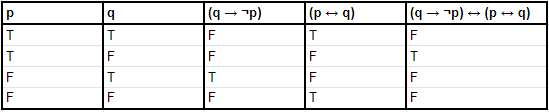
\includegraphics[scale = 0.55]{34E.PNG}
			\caption{Truth table for given proposition.}
		\end{figure}

\section*{Section 1.2}
	\subsection*{8 }
	$p$  "The user enters a valid password" \\
	$q$  "Access is granted" \\
	$r$  "The user has paid the subscription fee" 
		
	\subsubsection*{b) }
	"Access is granted($q$) whenever($\rightarrow$) the user has paid the subscription fee($r$) 
	and($\cdot$) enters a valid password($p$)."
		$$\boxed{q \rightarrow (r \cdot p)}$$

	\subsubsection*{c) }
		"Access is denied($q'$) if($\rightarrow$) the user has not paid the subscription fee($r'$)."
		$$\boxed{q' \rightarrow r'}$$

		\subsection*{44 }

		\begin{figure}[H]
			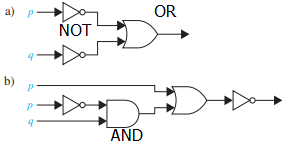
\includegraphics[scale = 0.55]{LG.PNG}
			\caption{Logic gates.}
		\end{figure}

	\subsubsection*{a) }

		$$\boxed{p'+q'}$$

	\subsubsection*{b) }

		$$\boxed{(p'q+p)'}$$

\section*{Section 1.3}
\subsection*{4 a) }

		\begin{figure}[H]
			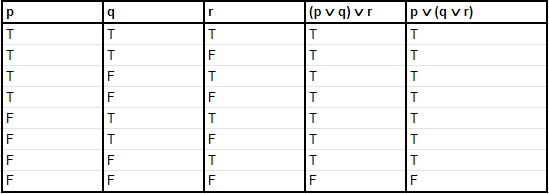
\includegraphics[scale = 0.55]{4A.PNG}
			\caption{Truth table for given proposition.}
		\end{figure}

		\subsection*{12 a) }

		\begin{figure}[H]
			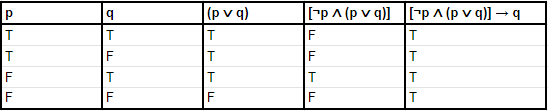
\includegraphics[scale = 0.55]{12A.PNG}
			\caption{Truth table for given proposition.}
		\end{figure}

	\subsection*{c) }

		\begin{figure}[h!]
			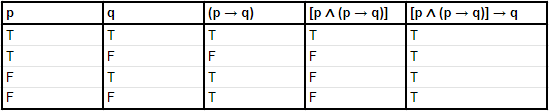
\includegraphics[scale = 0.55]{12C.PNG}
			\caption{Truth table for given proposition.}
		\end{figure}

		\subsection*{26 }

		\begin{figure}[H]
			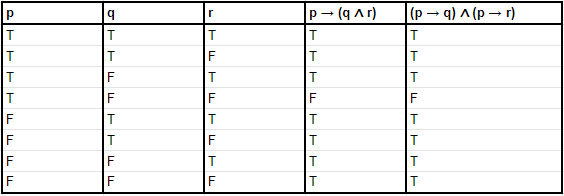
\includegraphics[scale = 0.55]{26.PNG}
			\caption{Truth table for given proposition.}
		\end{figure}

		$\therefore \boxed{(p \rightarrow q) + (p \rightarrow r) \equiv p \rightarrow (q + r)}$

\end{document}
